\subsection{Teilnahme und Login}

Beim ersten Laden der Anwendung soll eine Startseite aufgebaut werden, wie sie im Mock-Up \ref{fig:MockSignin} zu sehen ist. 
Hierbei soll der Nutzer zum einen die Möglichkeit haben bei einer Umfrage teilzunehmen. 
Dabei soll der Benutzer bzw. Student der an einer Umfrage teilnehmen möchte, einen \emph{Surveycode} wie \zb \emph{\texttt{OYZQGGXOF9}} eingeben, um an einer spezifischen Umfrage zu partizipieren. 
Anschließend wird der Benutzer auf die Umfrageseite weitergeleitet, auf der er die benötigten Felder ausfüllt (siehe Kap. \ref{ssec:konzept:client:umfrage}).
Hierbei soll der späteren Implementierung dieser Seite der Aspekt der mobilen Benutzung beachtet werden, da viele Benutzer eine Umfrage auf ihren mobilen Endgeräten durchführen. 
Bei allen anderen Seiten soll dieser Aspekt jedoch zunächst vernachlässigt werden.

\begin{figure}[H]
	\centering
	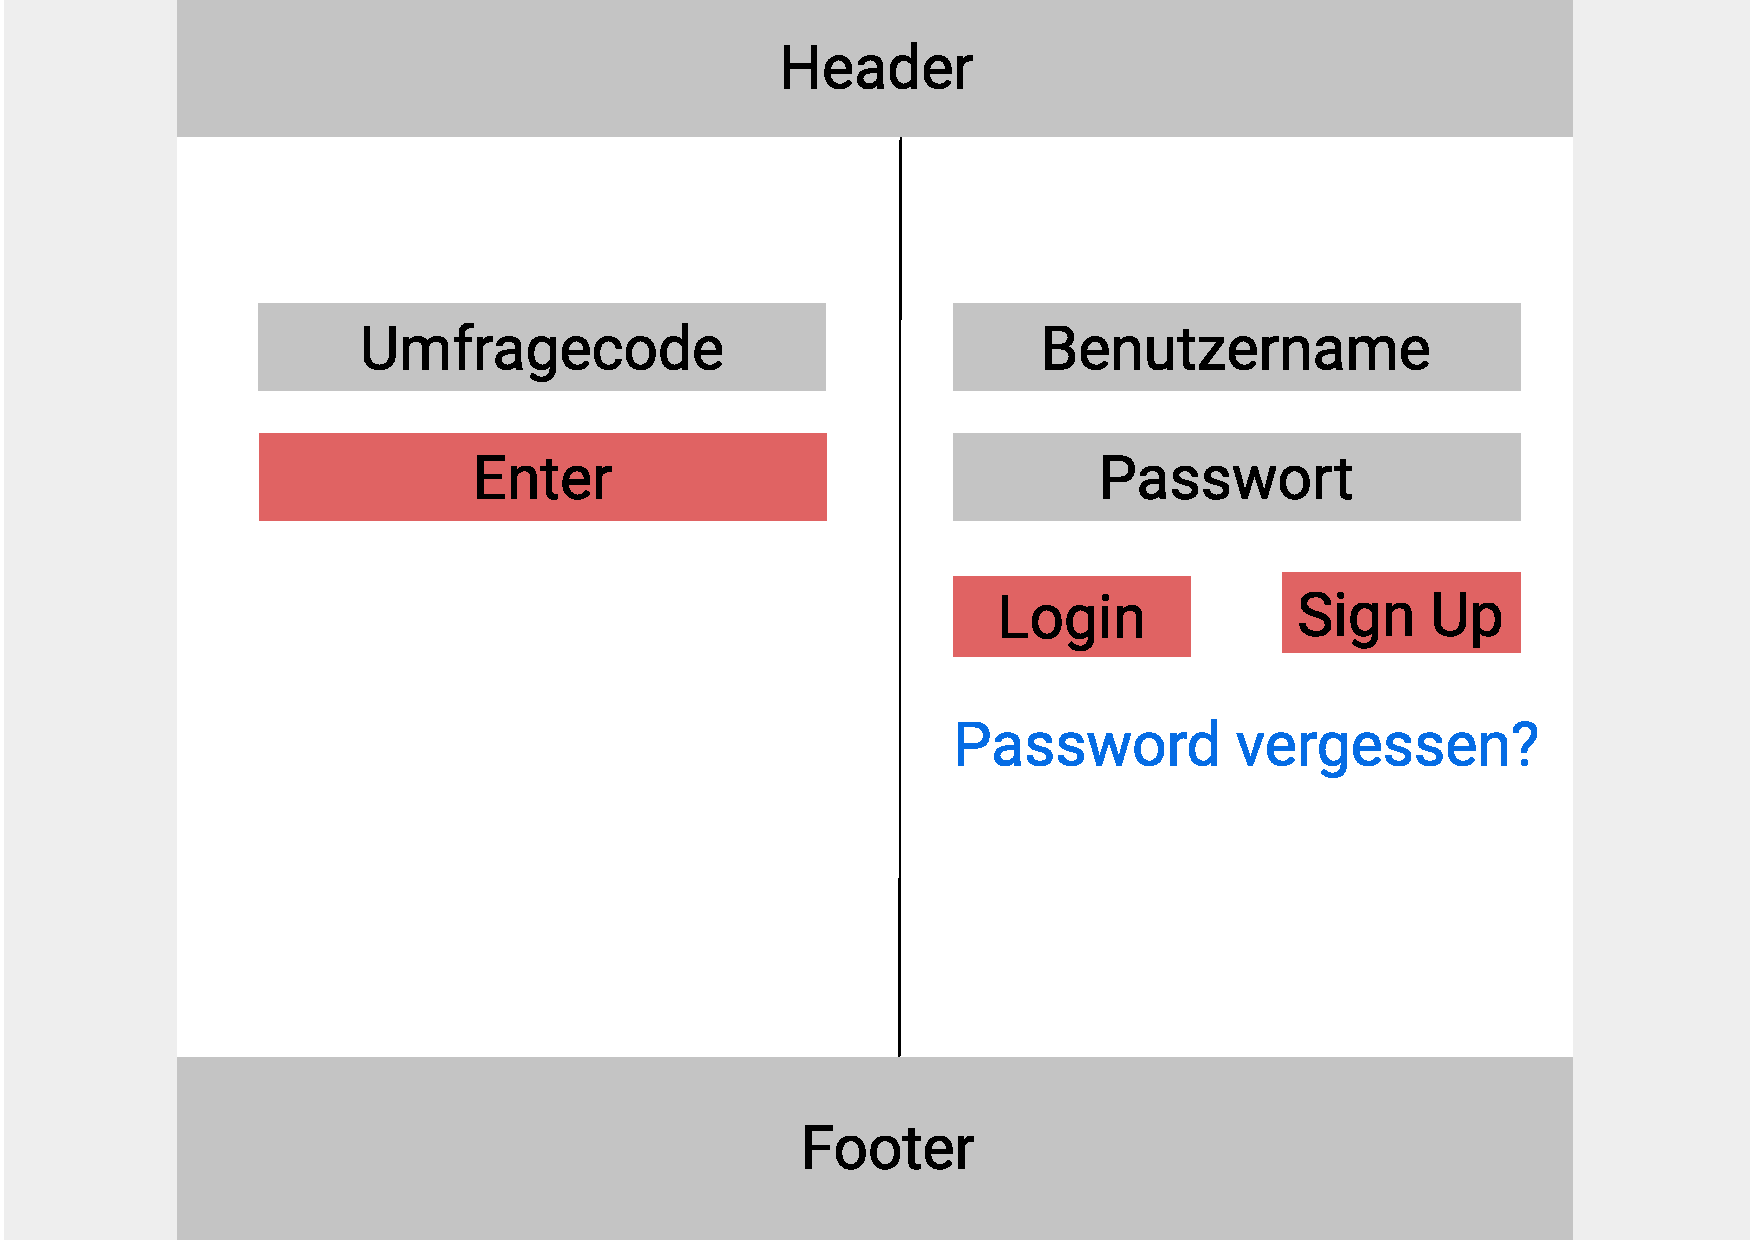
\includegraphics[width=0.7\textwidth]{img/konzeption/client/signin}
	\captionsetup{justification=centering, format=plain}
	\caption[Mock-Up der Startseite]{Mock-Up der Startseite \\\figma}
	\label{fig:MockSignin}
\end{figure}

Zum anderen soll der Benutzer die Möglichkeit besitzen, sich direkt in der Anwendung anmelden zu können.
Hierzu soll der \emph{Benutzername} und das \emph{Passwort} eines existierenden Benutzers eingegeben werden. 
Nach einer erfolgreichen Anmeldung soll der Benutzer auf die Dashboard-Seite weitergeleitet werden (siehe Kap. \ref{ssec:konzept:client:dashboard}).
Sollte kein valider Benutzer in der Anwendung vorhanden sein, so besteht die Möglichkeit auf den Button \emph{SignUp} zu klicken, um auf die Registierungsseite weitergeleitet zu werden (siehe Kapitel \ref{ssec:konzept:client:dashboard}).

